\subsection{Evaluation}
\label{vfree:sec:eval}


This section presents {\vfreename} evaluation. We first discuss {\vfreename} benefits for three real-world applications (\S\ref{vfree:ssec:real-world}), and then dive deeper into understanding {\vfreename} benefits using microbenchmarks (\S\ref{vfree:ssec:micro}). Next, we perform an ablation study of {\vfreename} design ideas (\S\ref{vfree:ssec:ablation}), discuss {\vfreename} scalability with increasing number of VMs (\S\ref{vfree:sec:eval-multi-vm}), and finally also discuss any associated costs of using {\vfreename} (\S\ref{vfree:ssec:cost}). 
% compared with vanilla system with vIOMMU on and off. 
% We use the pinned consumer configuration of {\vfreename}.
Unless stated otherwise, the system setup is the same as described in \S\ref{vfree:sec:inefficiencies}. 
% \saksham{Comback here to add overview}

\para{Measurement setups.}
% \schaic{All comments resolved. @Rachit please check.}
As mentioned in \S\ref{vfree:sec:inefficiencies}, we use two servers with Emerald Rapids processor architecture (which supports nested translation) directly connected to each other via $400$Gbps Nvidia ConnectX-7 NICs; this is to ensure that performance bottlenecks are not in the network. 
% The servers have  
%   with Intel Xeon Platinum 8592V CPUs and Intel Xeon Gold 6538Y+ CPUs respectively. 
% The former hosts our VMs, 
%   and the latter acts as client to send or receive traffic to the VM. 
  % a passive server engaged in Rx or Tx traffic 
  % \rachit{we have to be careful: each server does both Rx and Tx---right?}.  
% Each server has an Nvidia ConnectX-7 NIC; the two NICs connected to Ethernet with 400Gbps access link bandwidth.
These servers are 4-socket servers; each socket has
  32 physical cores, 252GB of memory and 150GB/s of memory bandwidth.
  % per-socket. 
The host server, guest VM, and client machines run with Ubuntu 22.04 and Linux v6.12.9. 
% \saksham{KVM/QEMU versions?} 
The VMs are hosted by QEMU v10.0 with nested translation~\cite{yiliu1765qemu}
and unmodified host OS (Linux 6.12.9).
% \saksham{Static pinning of vCPUs to physical cores to avoid interference.} 
We place the VMs on the NIC-local NUMA node to avoid any interference/degradation 
  due to cross-NUMA traffic.
Every vCPU of the VM is pinned to a separate physical core on the host to avoid interference. 
  We disable hyperthreading, CPU frequency scaling (we fix cores at their base frequency), and NUMA balancing for stable performance. 
Unless otherwise specified, we run all VMs with 32 vCPUs.
% We built a ebpf-based tool to measure the performance of guest and host OS.
% \saksham{if we get time, we should add error bars with stddev}.
% \schaic{We already have errors bars in the latest version @Saksham.}

We use Iperf3~\cite{iperf3} to generate network traffic and measure throughput.
We measure CPU utilization with sar~\cite{sar}.
We use eBPF probes to record the execution time and invocation counts of relevant kernel functions.
We measure VM exit counts, reasons, and time with perf~\cite{perf}.
We enable TCP Segmentation Offload (TSO), Generic Receive Offload (GRO), and adaptive Receive Flow Steering (aRFS)
to reflect high-performance networks. We run each experiment five times, and present the average results and standard deviation.



% We run the VM as receiver (Rx) 
%   and trasmitter (Tx) 
%   of network traffic, respectively, in two sets of experiments; this helps us isolate the impact of I/O memory protection on each setup. \rachit{this continues to be very confusing---saying that VM is the receiver of network traffic is incorrect since it also does Tx. We should precisely define what these two setups are: Rx receives large payloads and transmits ACKs; Tx transmits large payloads and receives ACKs;}
% Tx and Rx cases separately to isolate the impact of I/O memory protection on each datapath
%   (full-system results in \S\ref{vfree:sec:eval}). 
  % \rachit{readers may find this confusing---each server does both Rx and Tx.}
% later in eval section we run an end-to-end scenario where both kinds of traffic are running concurrently.
% \schai{: receive (Figure~\ref{vfree:fig:motivation-rx}) and transmit (Figure~\ref{vfree:fig:motivation-tx}).
% \noindent
% We increase the number of flows (each pinned to a core in the VM)
%   and compare throughput when running with
%   (1) vIOMMU off and (2) vIOMMU with strict memory protection (using nested translation).
% This section presents minimalist results to build an in-depth understanding of inefficiencies in strict intra-guest IO memory protection;
%   full results, including those for real-world applications, are 
%   in \S\ref{vfree:sec:eval}.


% \saksham{Let's not use the word nested in eval; we have already established earlier that we assume nested in this paper.}
% \saksham{we shouldn;t even use it in plots, draws unnecesary attention to nested vs shadow}

% We begin with real-world applications to highlight as much as $99\%$ throughput degradation with vIOMMU On.
% \saksham{let's not use such adjectives in papers :-); we just present the results and leave to the readers to infer its abysmal. we can simply say xyz percent degradation}
% \ikdelete{ and remarkable}
% \saksham{same comment as above for the word remarkable}
% \ikdelete{ improvements provided by \vfreename}
% With \name, we closely match the vIOMMU Off performance.
% We then analyze microbenchmark results for both Rx and Tx traffic to better understand the sources of degradation and how \vfreename mitigates them.
% Finally, we examine how each component of \vfreename\ contributes to overall performance, 
% as well as its resource overhead and the effect of key design choices.

\subsubsection{{\vfreename} Benefits for Real-world Applications}
\label{vfree:ssec:real-world}
We show the benefits of using {\vfreename} for three widely used high-performance 
    networked applications: 
    NGINX (a web server), 
    Redis (a distributed key-value store), 
    and SPDK (a userspace storage stack that uses Linux TCP stack for remote storage).
We use the same setup as earlier along with $9$KB MTU size. This helps maximize the application performance and avoid CPU becoming the performance bottleneck, when running with vIOMMU off. This allows us to focus mainly on IO memory protection-induced overheads when enabling vIOMMU and/or {\vfreename}. 
% To utilize the 400Gbps link bandwidth, we use 24 cores and a 9K MTU size~\cite{Rubin2024FastSafe}.
We use similar workloads for these applications as in prior work~\cite{Rubin2024FastSafe}; we describe them below inline with each application.  The NGINX workload most closely resembles the Tx-server setup, Redis to Rx-server setup, and SPDK has characteristics of both. 
% enabling a robust evaluation of {\vfreename} across traffic patterns.
% \schaic{@Saksham, I don't think Rx-host and Tx-host are standard terminology. 
% I changed to runs as receiver, transmitter, and concurrent receiver and transmitter.}
% \saksham{We should define the terminology in S3, and stick with it; I think a better terminology would be "Rx-host", "Tx-host" and host with concurrent Rx and Tx traffic}\ik{following the suggested terminology}.

\para{NGINX.} % Using nginx, we test \name's ability to handle Tx traffic.
% \saksham{we need to say why? give intuition that servers have majority Tx traffic because they serve HTTP GET requests from clients}. 
We run an NGINX instance inside a VM (which auto-scales to increasing load by spawning more worker threads). 
On the other host, we launch 24 clients, each pinned to a separate core. 
The clients use the \texttt{wrk} benchmark~\cite{wrk} to issue HTTP \texttt{GET} requests to the server.
We vary sizes of the requested webpage from 128 KB to 2 MB and report the aggregate throughput for each webpage size.

Figure~\ref{vfree:fig:nginx} shows over {$99\%$} throughput degradation with vIOMMU-on, 
    consistently across all evaluated webpage sizes.
\vfreebrand improves throughput by up to 147$\times$ over vIOMMU-on,
    and achieves close-to-vIOMMU-off performance for webpage sizes of 256\,KB and above, and within 7\% for 128\,KB.

% The gap at 128\,KB is due to smaller webpages causing more IO transactions per byte, 
%     increasing the number of unmap and invalidation requests vFree has to handle per unit of time. 
    
    % \ik{The simplest way to explain this is using CPU bottleneck. 128kB is already bottlenecked at vIOMMU off; lets say vFree has some extra CPU overhead => some degradation over vIOMMU off performance}


% \saksham{again, let's not use subjective terms---a value may be par for some and subpar for some :-). Just provide the results and let people infer.} 
% nginx Tx\saksham{no need to repeat "Tx" again} performance with vIOMMU on. 
% The throughput degradation is consistent across all webpage sizes, with over $99\%$ throughput degradation
% \saksham{same feedback as earlier for times vs percentage}\ikdelete{. This degradation is consistent across all webpage sizes}\saksham{repeated statement}. 

% Figure~\ref{vfree:fig:nginx} exhibits subpar
% \saksham{again, let's not use subjective terms---a value may be par for some and subpar for some :-). Just provide the results and let people infer.} 
% nginx Tx\saksham{no need to repeat "Tx" again} performance with vIOMMU on. 
% The throughput degradation is consistent across all webpage sizes, with over $99\%$ throughput degradation
% \saksham{same feedback as earlier for times vs percentage}\ikdelete{. This degradation is consistent across all webpage sizes}\saksham{repeated statement}. 
% Using {\vfreename}, the throughput is restored to near-vIOMMU-off performance\saksham{instead of phrases like throughput is restored, use simpler to-the-point phrases, like \vfreename provides close-to-vIOMMU-disabled performance}\ikdelete{, with strict invalidation policy enabled}\saksham{no need to repeat this again}.

\para{Redis.} 
% Using Redis, we test \name's ability to handle Rx traffic.
We run 24 Redis server instances inside a VM, with one instance per core. 
We use redis-benchmark~\cite{redis-benchmark} to launch an equal number of client instances on the other host,
    each sending \texttt{SET} requests to a corresponding server instance. 
We vary the \texttt{SET} value size from 8 KB to 256 KB, and 
    for each value size, we follow prior work~\cite{Rubin2024FastSafe} 
    to tune the number of parallel connections, client threads, and request batch size
    and report the optimal aggregated throughput.


Figure~\ref{vfree:fig:redis} shows that vIOMMU-on
% \ikdelete{ with strict protection}\saksham{we dont have to say strict protection again, just say it once during setup that you assume this, unless specified otherwise} 
can cause up to $98\%$ throughput degradation
% \saksham{I think we should use percentage degradation, instead of xyz times} 
with higher degradation for smaller \texttt{SET} value sizes (<= 64KB).
% \ikdelete{, with smaller }
% \saksham{smaller values of what?}\ikdelete{ leading to even worse performance}.
\vfreebrand improves throughput by up to 74$\times$ over vIOMMU-on 
    and achieves close-to-vIOMMU-off performance, with at most 6\% gap.



\begin{figure}[H]
    \centering
    \begin{subfigure}[b]{0.32\textwidth}
        \centering
        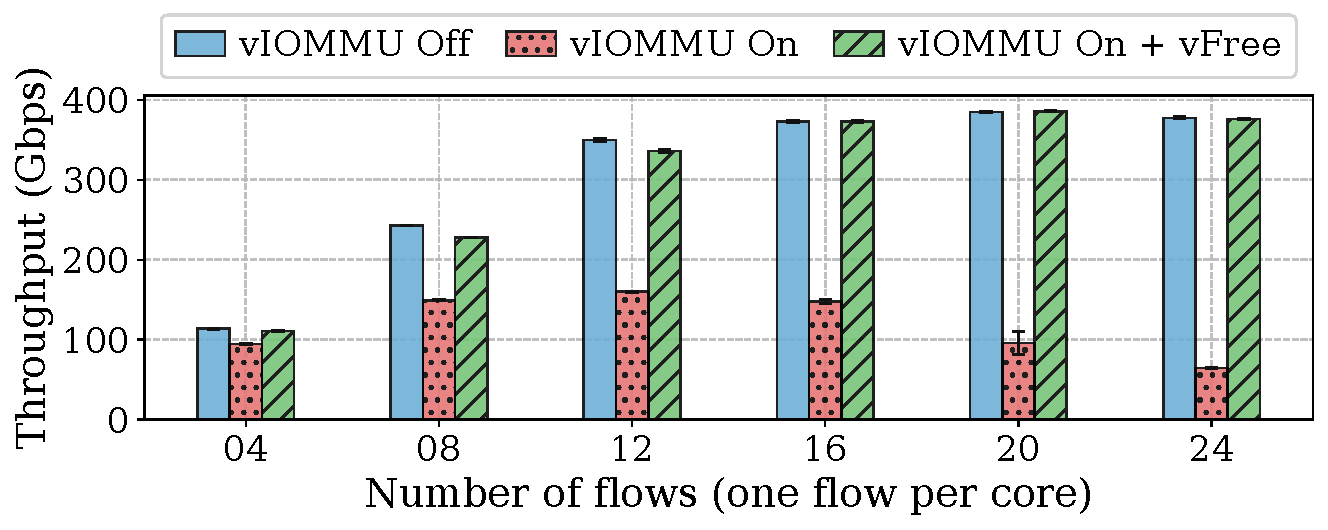
\includegraphics[width=\textwidth]{figures/eval_core_exp-tput.pdf}
        \caption{Throughput}
        \label{vfree:fig:eval-core-tput}
    \end{subfigure}
    \hfill
    \begin{subfigure}[b]{0.32\textwidth}
        \centering
        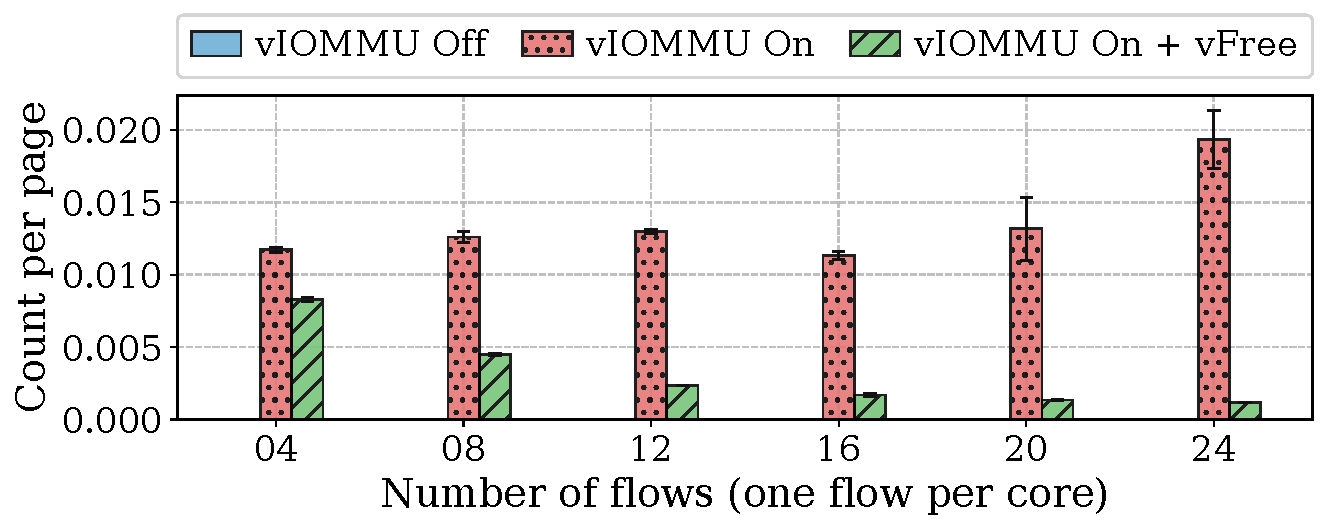
\includegraphics[width=\textwidth]{figures/eval_core_exp-qi_submit_sync-count_per_page.pdf}
        \caption{IR-SUB count per page}
        \label{vfree:fig:eval-core-qi}
    \end{subfigure}
    \hfill
    % \begin{subfigure}[b]{0.32\textwidth}
    %     \centering
    %     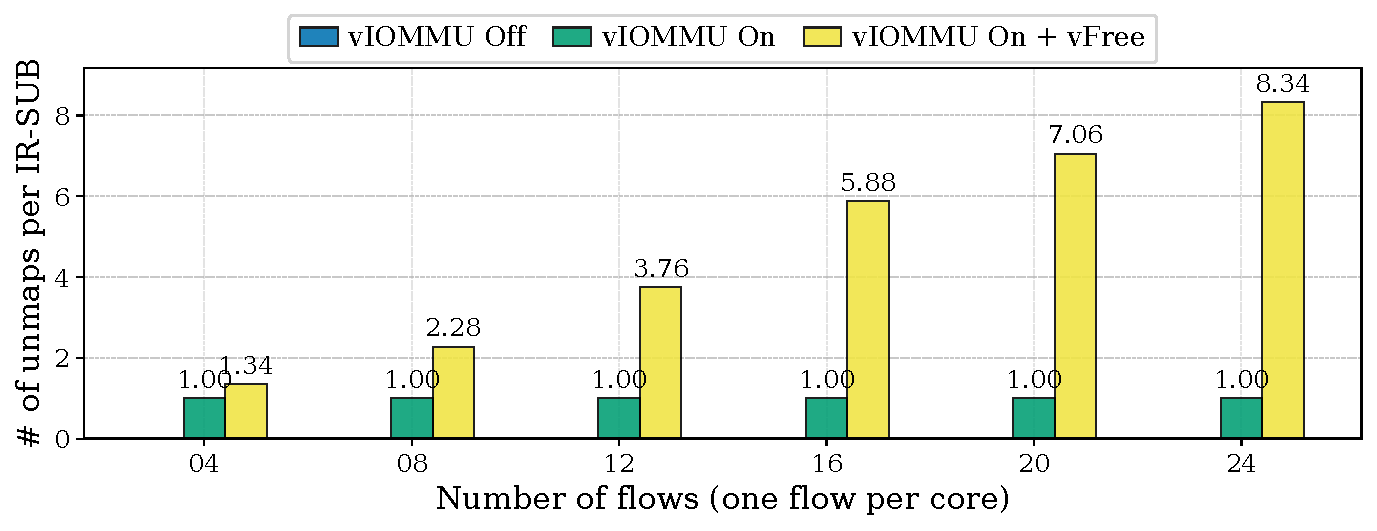
\includegraphics[width=\textwidth]{figures/eval_core_exp-unmap_to_qi_submit_ratio.pdf}
    %     \caption{Number of IR per IR-SUB}
    %     \label{vfree:fig:eval-core-unmap-ratio}
    % \end{subfigure}
    % \hfill
    \begin{subfigure}[b]{0.32\textwidth}
        \centering
        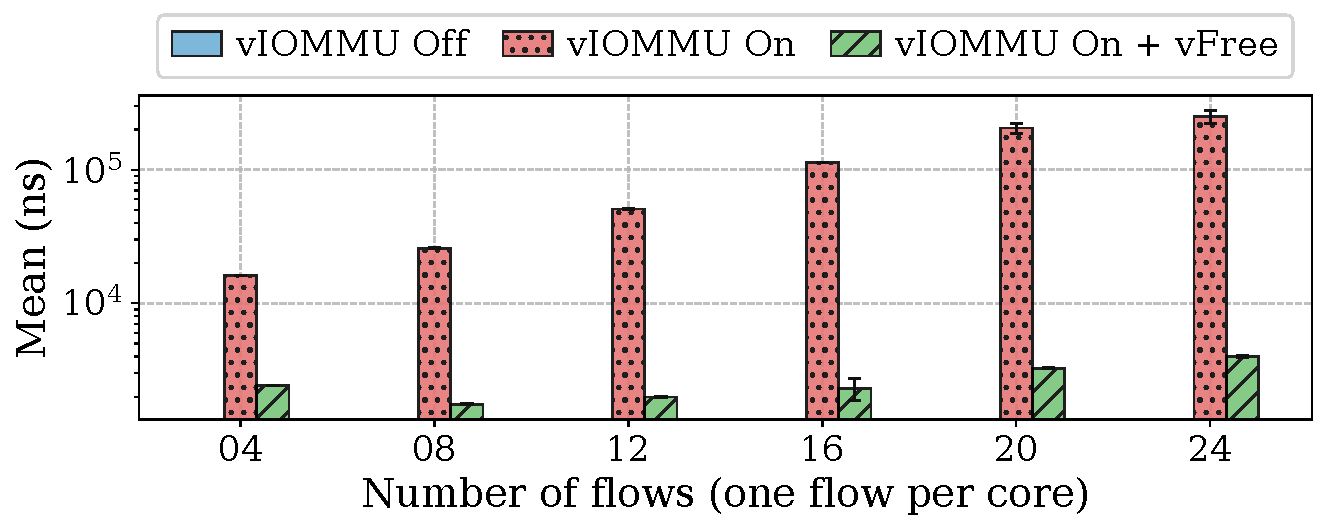
\includegraphics[width=\textwidth]{figures/eval_core_exp-cache_tag_flush_range-mean_ns.pdf}
        \caption{IR processing latency per unmap}
        \label{vfree:fig:eval-core-flush}
    \end{subfigure}
    \caption{\small {\bf Rx-server.} \vfreename{} achieves up to $4.9\times$ Rx throughput improvement over vIOMMU-on.}
%    \schaic{c)'s caption is a bit hard in one line. See text for detailed definition.}}
    \label{vfree:fig:eval-core}
\end{figure}

\begin{figure}[H]
    \centering
    \begin{subfigure}[b]{0.32\textwidth}
        \centering
        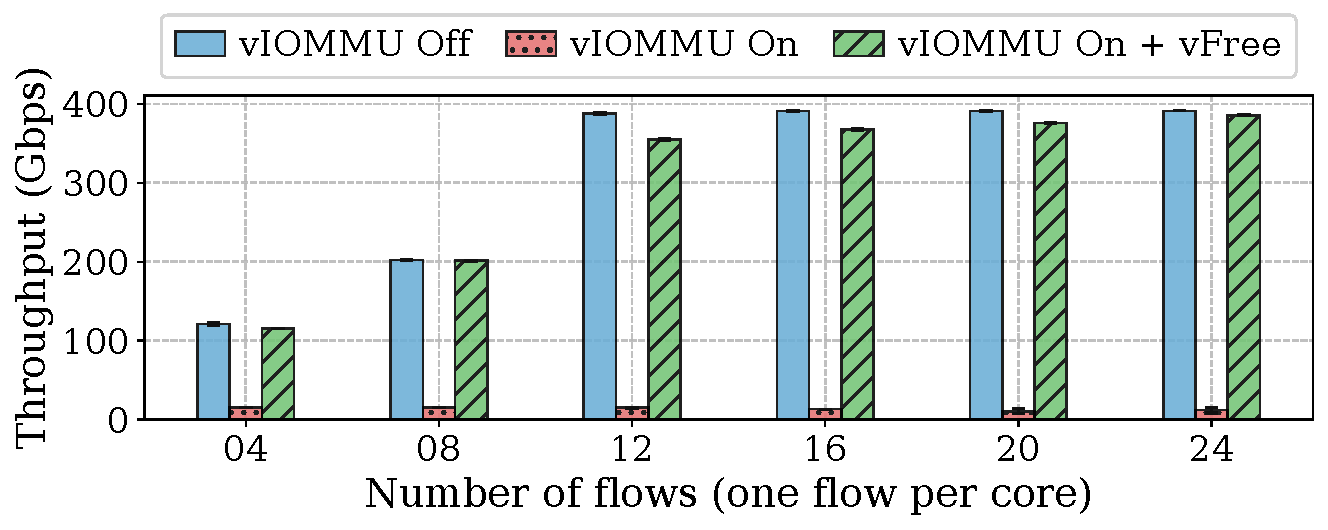
\includegraphics[width=\textwidth]{figures/tx-ebpf-tput.pdf}
        \caption{Throughput}
        \label{vfree:fig:tx-tput}
    \end{subfigure}
    \hfill
    \begin{subfigure}[b]{0.32\textwidth}
        \centering
        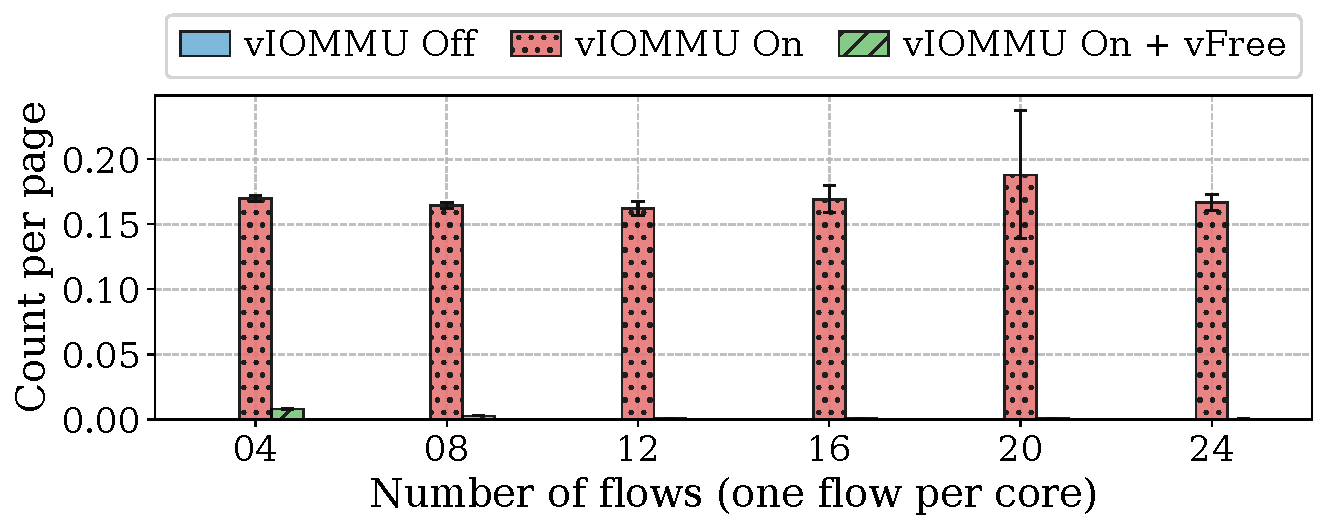
\includegraphics[width=\textwidth]{figures/tx-ebpf-qi_submit_sync-count_per_page.pdf}
        \caption{IR-SUB count per page}
        \label{vfree:fig:tx-qi}
    \end{subfigure}
    \hfill
    \begin{subfigure}[b]{0.32\textwidth}
        \centering
        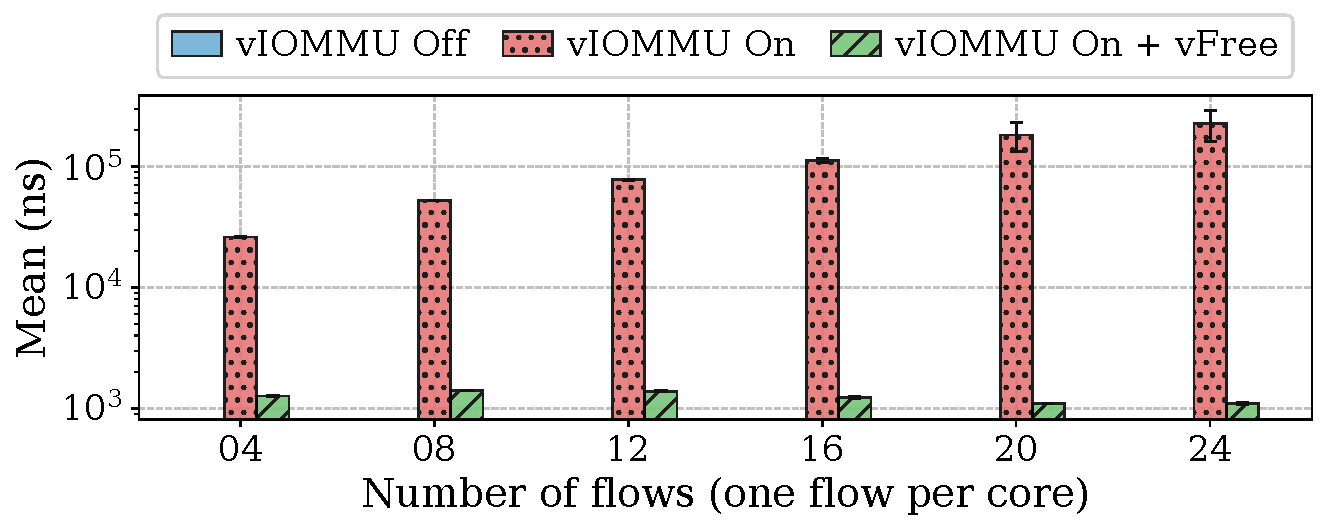
\includegraphics[width=\textwidth]{figures/tx-ebpf-cache_tag_flush_range-mean_ns.pdf}
        \caption{IR processing latency per unmap}
        \label{vfree:fig:tx-flush}
    \end{subfigure} 
%    \caption{Tx microbenchmark (one flow per core): \vfreename{} achieves up to $36\times$ throughput improvement over the vIOMMU On configuration
%    by reducing IR-SUB count per page and IOTLB invalidation overhead.
    \caption{\small {\bf Tx-server.} \vfreename{} achieves up to 36$\times$ Tx throughput improvement over vIOMMU-on.}
    \label{vfree:fig:tx}
\end{figure}

\para{SPDK.} 
% To stress-test \name's ability to handle concurrent Rx and Tx traffic,
% We configure SPDK to serve a mix of read and write IO requests over TCP.
% We use SPDK to evaluate a workload where the VM concurrently receives and transmits network traffic, 
% thereby stressing both Rx and Tx datapaths. 
We create a RAM-backed block device and run 24 SPDK server instances inside a VM, one per core.
On the other host, we run an equal number of \texttt{fio}~\cite{fio} clients, 
    each generating a workload with 60\% reads and 40\% writes and an IO depth of 8\footnote{We opt for 60:40 read-write ratio and IO depth 8 to avoid memory bandwidth bottleneck. 
    In general, writes consume twice the memory bandwidth 
    of reads, as each write involves a memory read followed by a memory write.}.
We vary the block size from 32 KB to 512 KB and report the aggregate throughput.
% \saksham{Try to give more context as to why we create so much fuss about mixed workload---that there would be more no. of unmap requests the IOMMU will have to serve?}\ik{We do not have a good reason besides stressing both Rx and Tx datapaths, and creating a more realistic scenario. The original plan was to use Rx (SET) only, but that lead to memory BW bottleneck.}

Figure~\ref{vfree:fig:spdk} shows over 97\% throughput degradation 
    with vIOMMU-on across all block sizes.
\vfreebrand improves throughput by up to 82$\times$ over vIOMMU-on and 
    achieves close-to-vIOMMU-Off performance, with at most an 8\% gap.

% The gap of 8\% happens at the smallest block size of 32\,KB which 
    % has more overhead (similar to small webpages in NGINX).

% \vspace{0.1in}
% \noindent
% The small, 6-8\%, performance gap is observed only for the smallest-sized IO requests in all three applications. This is because CPU became the bottleneck for these cases even for vIOMMU-off, and additional CPU cycles spent on map/unmap operations with {\vfreename} led to slightly lower throughput. 
    
% Smaller block sizes result in more IO transactions per byte, 
%    increasing the number of unmap calls and invalidation requests that vFree has to handle per unit of time.}

% \textbf{SPDK.} We use SPDK to evaluate concurrent Rx and Tx traffic\saksham{use consistent terminology defined earlier}, thereby stressing datapaths. To configure SPDK, we first create a\ikdelete{ "malloc"}\saksham{"malloc" not needed} block device (backed by RAM) to serve \ikreplace{read and write}{IO} requests over TCP\saksham{say IO requests here; later we show IO workload with read:write ratio}. We then run 24 SPDK server instances inside the VM, with one instance pinned to each core. The other host\saksham{terminology} runs an equal number of \texttt{fio} \cite{fio} clients, each generating a workload with 60\% reads and 40\% writes\saksham{why did we use 60:40? is it something standard workload, or used in prior work? Why not just 50:50?}\ik{Why not 50:50 addressed in footnote. In fact, we use a mixed workload only to avoid memory BW bottleneck}\footnote{We use a 60:40 split of reads v/s writes to avoid memory bandwidth bottleneck. Writes consume twice the memory bandwidth of reads as each write involves a memory read followed by a memory write.} at an IO depth of 8\footnote{We choose an IO depth of 8, as increasing it further does not improve throughput due to memory bandwidth bottlenecks on the SPDK server.}\saksham{why 8? is it the knee point?}. We vary the block size from 16 KB to 512 KB and report the aggregate throughput across reads and writes.
% \saksham{Try to give more context as to why we create so much fuss about mixed workload---that there would be more no. of unmap requests the IOMMU will have to serve?}\ik{We do not have a good reason besides stressing both Rx and Tx datapaths, and creating a more realistic scenario. The original plan was to use Rx (SET) only, but that lead to memory BW bottleneck.}

\subsubsection{Understanding {\vfreename} Benefits}
\label{vfree:ssec:micro}
% Section~\ref{vfree:sec:inefficiencies} presents the overhead of memory protection with vIOMMU.

To better understand the reasons for {\vfreename} performance benefits, we also evaluate {\vfreename} using microbenchmarks. We use Iperf3~\cite{iperf3} to generate network traffic and measure throughput. We use similar setup as in \S\ref{vfree:sec:inefficiencies}, running same sets of controlled experiments, with the VM acting as the Tx-server and Rx-server, respectively. This enables us to analyze the individual impact of these setups on {\vfreename} performance.



\para{Rx-server.} 
% \ikdelete{ We evaluate this setup under the three configurations described in \S\ref{vfree:sec:eval}}
% \saksham{last line is not necessary; already mentioned in setup}
% \ikdelete{. Enabling vIOMMU in strict mode significantly degrades performance compared to vIOMMU off}
% \saksham{this was already discussed earlier in S3, when discussing fig 2}
% In contrast, \vfreename restores throughput to near-vIOMMU-off level.
% \saksham{"restores"}
% \ikdelete{ while preserving the same security guarantees as strict invalidation policy}
% \saksham{this repetitive; and even then also inconsistent, sometimes it says strict protection, sometimes strict invalidation policy}
% Overall, \vfreebrand achieves up to a $83\%$ throughput improvement over the vIOMMU on configuration.
As shown in Figure~\ref{vfree:fig:eval-core-tput}, {\vfreename} improves throughput by up to $4.9\times$ in comparison to vIOMMU-on, 
matching closely to vIOMMU-off performance (with a maximum gap of <6\%).
The key contributor to this throughput improvement is the reduction of IR-SUB operations per page transferred over network. As shown in Figure~\ref{vfree:fig:eval-core-qi}, {\vfreename} reduces the IR-SUB count per page by up to 82\%. Recall from \S\ref{vfree:sec:background-datapath}, each IR-SUB operation requires an unavoidable VM exit, hence, reduction in IR-SUB count translates to a similar reduction in VM exits per page. {\vfreename} achieves this reduction using two design ideas. One-for-many invalidations allow using a single IR-SUB to invalidate concurrently prepared IRs across multiple cores---hence, we see lower IR-SUB counts per page with increasing numbers of cores in Figure~\ref{vfree:fig:eval-core-qi}. Furthermore, deferred free page allows each core to prepare multiple IRs that can be concurrently processed by a single IR-SUB operation. This is achieved by avoiding busy waiting by each core until successful invalidation for each prepared IR, and hence reducing the time spent on IR processing by the core after {\tt unmap}. Figure~\ref{vfree:fig:eval-core-flush} shows the average time spent by application core on IR processing: while vIOMMU-on incurs large IR processing time due to incurring all---\CodeIn{cache\_lock} contention, IR-PREP and IR-SUB overheads,  {\vfreename} avoids lock contention due to its per-CPU locks, and avoids IR-SUB due to deferred free page, and observes up to 99.9\% reduction in IR processing time. 

\para{Tx-server.} 
Figure~\ref{vfree:fig:tx-tput} shows that {\vfreename} achieves up to 36$\times$ throughput improvement over vIOMMU-on,
closely matching vIOMMU-off (with the largest gap of <9\%). The root cause of {\vfreename} benefits are similar to those discussed earlier for the Rx-server case. We briefly discuss the reason behind the relatively larger throughput gains in the Tx-server case. This is because of larger number of unmaps per page performed in Tx datapath (recall that Linux's page pool optimization does not apply to Tx datapath; \S\ref{vfree:sec:background-datapath}). Due to much larger number of unmaps per page, {\vfreename} is able to enqueue much larger number of IR descriptors into the IO-domain queue, which can be submitted using a single IR-SUB---hence further reducing the IR-SUB count per page (as evident from Figure~\ref{vfree:fig:tx-qi}). This leads to relatively larger reductions in VM exits per page for Tx-server case, improving the relative performance gains.

% Both \optOne{} and DFP contribute significantly to the improvements\ik{but in ablation we say DFP is the primary; which is accurate; would be good to mention somewhere that primary contributors to performance are different in Tx and Rx}.
% \optOne{} aggregates multiple invalidation requests into a single IR-SUB operation,
% reducing the IR-SUB count per page by $300\times$ (Figure~\ref{vfree:fig:tx-qi}).
% DFP further increases the batching factor by releasing producer threads from waiting for invalidation to complete,
% reducing the average time the guest spends in the IOMMU subsystem by over 200$\times$ (Figure~\ref{vfree:fig:tx-flush}).


% With vanilla Linux and mlx5 driver, every transmitted socket buffer triggers at least one map, 
%     one unmap, and one cache invalidation---exerting
%     high pressure on the IOMMU subsystem and resulting in a 15$\times$ 
%     higher IR-SUB count per page compared to the Rx case (Figure~\ref{vfree:fig:tx-qi}).

% \schaic{Consider Removing fig:stress-qi and fig:stress-flush if we are short of space.}


% Rather than stalling on each invalidation, producer threads enqueue their requests and continue execution.

% Reduction by by up to 99.9\%
% the near-total reduction confirms that {\vfreename} effectively eliminates both bottlenecks.

% through \optOne{}---which aggregates multiple invalidation requests into a single IR-SUB operation. 


% This batching scales with parallelism: the number of invalidation requests handled per IR-SUB grows linearly from 1.3 to 8.3 as the number of active cores increases.

% DFP further enables asynchronous invalidation without losing strict safety guarantees.


% As shown in Figure~\ref{vfree:fig:eval-core-flush}, {\vfreename} reduces the average time the guest OS spends in the IOMMU subsystem for IOTLB invalidation by up to 99.9\%,
% almost completely eliminating invalidation overhead.
% This metric subsumes locking contention and IR-SUB operation in Figure~\ref{vfree:fig:lock-contention};
% the near-total reduction confirms that {\vfreename} effectively eliminates both bottlenecks.

% \ik{does not match with ablation study data where we say atmost 3 in a batch; it is important to clarify that these numbers are with DFP which can increase batch size} 

% In this experiment, the VM acts as receiver while the client serves as sender.
% \ikdelete{ We evaluate this setup under the three configurations described in \S\ref{vfree:sec:eval}}\saksham{last line is not necessary; already mentioned in setup}\ikdelete{. Enabling vIOMMU in strict mode significantly degrades performance compared to vIOMMU off}\saksham{this was already discussed earlier in S3, when discussing fig 2} In contrast, \vfreebrand restores\saksham{"restores"} throughput to near-vIOMMU-off level\ikdelete{ while preserving the same security guarantees as strict invalidation policy}\saksham{this repetitive; and even then also inconsistent, sometimes it says strict protection, sometimes strict invalidation policy}. Overall, \vfreebrand achieves up to a $83\%$ throughput improvement over the vIOMMU on configuration.

% A key factor behind the substantial throughput improvement is the reduction in VM exits, due to fewer invalidation requests. As shown in Figure~\ref{vfree:fig:eval-core-qi}, \vfreebrand lowers invalidations per page by up to $82\%$ through delegated invalidation: requests from multiple cores are aggregated, and a single core issues a batched invalidation request. Importantly, a batched invalidation to the IOMMU hardware takes roughly the same time as an individual request, so the duration of each VM exit remains unchanged. Another contributing factor is the reduction in the total time the guest OS spends in the IOMMU subsystem, enabled by the deferred free page (DFP) optimization. During a VM exit, only the issuing core is blocked while waiting for the invalidation to complete, whereas other cores can simply enqueue their invalidation requests and continue execution without stalling. As shown in Figure~\ref{vfree:fig:eval-core-flush}, \vfreebrand reduces the average time that guests OS spends in the IOMMU subsystem by up to $99.9\%$, nearly eliminating the overhead of IOTLB invalidation.

% In Figure~\ref{vfree:fig:stress}, we stress-test \vfreebrand by varying the number of flows per core on a 24-core configuration. Combining results from Figure~\ref{vfree:fig:eval-core} and Figure~\ref{vfree:fig:stress}, we observe that \vfreebrand scales well with both increasing core counts and higher number of per-core flows. Across all scenarios, \vfreebrand closely matches vIOMMU off performance.

% A key factor behind the substantial throughput improvement is the reduction in VM exits, due to fewer invalidation requests.

% text on count per page.
% A key factor behind the substantial throughput improvement is the reduction in VM exits, due to fewer invalidation requests. 
% As shown in Figure~\ref{vfree:fig:eval-core-qi}, \vfreebrand lowers invalidations per page by up to $82\%$ through delegated invalidation:
%  requests from multiple cores are aggregated, and a single core issues a batched invalidation request. 
%  Importantly, a batched invalidation to the IOMMU hardware takes roughly the same time as an individual request, so the duration of each VM exit remains unchanged. Another contributing factor is the reduction in the total time the guest OS spends in the IOMMU subsystem, enabled by the deferred free page (DFP) optimization. During a VM exit, only the issuing core is blocked while waiting for the invalidation to complete, whereas other cores can simply enqueue their invalidation requests and continue execution without stalling. As shown in Figure~\ref{vfree:fig:eval-core-flush}, \vfreebrand reduces the average time that guests OS spends in the IOMMU subsystem by up to $99.9\%$, nearly eliminating the overhead of IOTLB invalidation.



% \schaic{I have a figure for this (eval\_core\_exp-unmap\_to\_qi\_submit\_ratio.pdf). Shall we replace it with current Figure~\ref{vfree:fig:eval-core-qi}?}

% Such "one-for-many" optimization completely changes the story of IR-PREP and IR-SUB serlization 
    % in vanilla vIOMMU on.

% aggregating multiple invalidation requests into a single IR-SUB operation.
% As we discussed in \S\ref{vfree:sec:inefficiencies},
% vIOMMU on incurs significant overhead because it couples IR-PREP and IR-SUB operations,
% and serializes them across all network threads.
% A key factor behind the substantial throughput improvement is the reduction 
% in IR-SUB operation per page.
% in VM exits, due to fewer invalidation requests. 
% As shown in Figure~\ref{vfree:fig:eval-core-unmap-ratio}, 
% vIOMMU performs one IR-SUB operation for each unmap call which corresponds to one IR.
% the cross-thread serialization of IR-PREP and IR-SUB operations in 
% \vfreename lowers invalidations per page by up to $82\%$ through delegated invalidation: 
% invalidation requests from multiple producer threads are aggregated, 
% and a single consumer thread issues one IR-SUB operation tha handles all the aggregated requests. 
% Importantly, a batched invalidation to the IOMMU hardware takes roughly the same time as an individual request, 
% so the duration of each VM exit remains unchanged. 


\if 0
We further stress-test \vfreename{} by scaling up to eight concurrent flows across 24 cores (see Figure~\ref{vfree:fig:stress}
    in the appendix).
Under excessive loads, \vfreename{} maintains throughput within 1\% of vIOMMU-off performance.
Combining the results from Figures~\ref{vfree:fig:eval-core} and~\ref{vfree:fig:stress}, 
we observe that \vfreename{} scales robustly with both increasing core counts and flows per core. 
\fi

% reduces the number of invalidation requests by over $300\times$ (Figure~\ref{vfree:fig:tx-flush}) through batching. 

% Combined with DFP, it also reduces the time the guest OS spends in the IOMMU subsystem by over $200\times$ (Figure~\ref{vfree:fig:tx-qi}), as cores can simply enqueue invalidation requests and avoid waiting for IOTLB invalidation to complete.


% \textbf{\vfreename\ performance with Tx traffic.} We use the same setup as in \S\ref{vfree:sec:inefficiencies}. 
% In this experiment, the VM acts as sender and the client as receiver, with traffic generated using Iperf.
% Figure~\ref{vfree:fig:tx} evaluates the setup under the same three configurations as described in \S\ref{vfree:sec:eval}. 


% This is because the vIOMMU on configuration incurs a much higher number of invalidations per page for Tx traffic (Figure~\ref{vfree:fig:tx-qi}) than for Rx traffic (Figure~\ref{vfree:fig:eval-core-qi}). The increase is driven by more frequent \CodeIn{map()}/\CodeIn{unmap()} operations, as discussed in \S\ref{vfree:sec:linux-opt}, leading to more VM exits and greater time per core spent waiting on the \CodeIn{cache\_lock}.

% As shown in Figure~\ref{vfree:fig:tx-tput}, the throughput degradation between vIOMMU Off and the vIOMMU On configuration is significantly more pronounced in the Tx case. Despite this, \vfreename restores throughput to near-vIOMMU-Off level. In fact, \vfreename achieves up to $98\%$ throughput improvement over the vIOMMU On configuration. Similar to the Rx case, this improvement originates from two key optimizations---delegated invalidation and DFP optimization. Delegated invalidation reduces the number of invalidation requests by over $300\times$ (Figure~\ref{vfree:fig:tx-flush}) through batching. Combined with DFP, it also reduces the time the guest OS spends in the IOMMU subsystem by over $200\times$ (Figure~\ref{vfree:fig:tx-qi}), as cores can simply enqueue invalidation requests and avoid waiting for IOTLB invalidation to complete.


\subsubsection{{\vfreename} Ablation Study}
\label{vfree:ssec:ablation}

We quantify the contributions of 
\optOne{}, deferred free page,
and other {\vfreename} code optimizations (\S\ref{vfree:sec:other-opt}) to overall throughput for both Rx- and Tx-server setups.
In our analysis, we vary the number of cores from 4 to 24, 
    each running one flow, and report the corresponding throughput.

\para{Tx-server.} Figure~\ref{vfree:fig:ablation-tx} shows that code optimizations provide a modest contribution in overall gains. One-for-many invalidations improve the throughput further by {1.1-2.9$\times$}, with increasing gains with larger core count. This is expected since more cores enable {\vfreename} to invalidate more concurrent IRs via single IR-SUB. Deferred free page, however, provides most significant contribution to throughput gains---{2.9 to 5.6$\times$}. Without deferred free page, each core stays blocked after IR-PREP until successful invalidation completion for the IR. When no longer constrained to busy wait with deferred free page, each core can continue execution of the future unmaps. And since in Tx-server setup, as discussed earlier, there are a large number of unmaps generated per core, this unblocking of cores results in significant throughput gains. 




% DFP is the primary contributor to throughput gains for Tx traffic.
% As discussed in \S\ref{vfree:sec:linux-opt},
% the Tx datapath invokes significantly more \CodeIn{map()}/\CodeIn{unmap} operations,
% resulting in a much higher rate of invalidation requests.
% While \optOne{} reduces the number of VM exits by batching these invalidations,
% it stalls threads that generate invalidation requests until its invalidation is completed (to mantain strict safety guarantee).
% % it creates a bottleneck:
% % all cores that contribute requests to a batch must synchronously wait for the invalidation to complete.
% As a result, \optOne{} alone fails to scale throughput with increasing core count.
% Although batching opportunities improve with more cores,
%     the wait for invalidation caps the throughput to the rate of IR-SUB operations.\ik{we can probably start by saying that one-to-many alone is not sufficient due to large batch sizes and more cores blocked, and then we say that DFP removes waiting so performance improves}

\para{Rx-server.} 
Unlike Tx-server, Figure~\ref{vfree:fig:ablation-rx} shows that for Rx-server, one-for-many invalidations provides more significant contribution to overall gains. This is due to relatively lower numbers of unmaps per page observed in the Rx-datapath: there is relatively smaller performance impact of unblocking the cores using deferred free page due to larger inter-arrival times between unmap requests within each core. 


% Different from Tx, both \optOne{} and DFP 
%     contribute significantly to the performance improvements 
%     over vIOMMU-on by reducing the number of VM exits. 
% % Since each invalidation triggers a VM exit, 
% % aggregating multiple invalidation requests into a single IR-SUB operation significantly lowers the overall VM exit overhead.
% Specifically, \optOne{} opportunities naturally increase with core count, 
%     improving throughput by 1.5$\times$ at 12 cores and up to 4.8$\times$ at 24 cores.
% Applying DFP atop \optOne{} yields additional gains.
% The relatively modest improvement is expected\ik{imo we see modest gains only because there is no scope to improve on top of vIOMMU off, so DFP simply fills the gap}: at high Rx traffic rates, 
%     few unmap operations---and thus few invalidation requests---are generated.
% In our profiling, 99.9+\% of IOMMU operations are generated by the Tx datapath, which primarily sends ACKs to the sender.
% % , thanks to the page pool optimization (\S\ref{vfree:sec:linux-opt}).
% With a low invalidation rate, only a small number of cores are blocked at a time, waiting for invalidation to complete.\ik{the fact that "one-to-many invalidations achieve good improvement due to small batch sizes and fewer cores blocked" is not clearly conveyed here}
% \if 0 % save space
% Consequently, \optOne{} alone achieves 71\% of vIOMMU Off performance at 12 cores and 99\% at 24 cores.
% DFP closes the residual gap by deferring page reclamation, 
% allowing even those few blocked cores to enqueue their requests and continue without stalling.
% \fi 
% % ---but the additional benefit is inherently limited when synchronization pressure is already low.


% \textbf{Rx Ablation Study.} 
% As shown in Figure~\ref{vfree:fig:ablation-rx}, SBI mitigates a large fraction of the performance lost with vIOMMU On. This improvement stems from batching invalidation requests, which reduces the number of VM exits. Since each invalidation triggers a VM exit, amortizing them across batches significantly lowers the overall VM exit overhead. Moreover, batching opportunities naturally increase with core count. As a result, the relative benefit of SBI grows with scale, improving throughput by \textasciitilde35\% at 12 cores and up to \textasciitilde83\% at 24 cores.

% Applying DFP on top of SBI yields additional, but smaller, gains. The relatively modest improvement is expected, as SBI already addresses the primary bottleneck, while DFP serves to close the residual gap. \leshna{I agree with the first line, but not the reason, why does SBI address the primary bottleneck, a small callback of we have low number of unmap may be helpful. Basically TX and RX explanation should complement} Specifically, DFP reduces time spent in the guest IOMMU subsystem by deferring page reclamation work. During a VM exit, only the issuing core is blocked, while other cores can enqueue invalidation requests and continue execution without stalling.


\begin{figure}[H]
    \centering
    \begin{subfigure}[b]{\columnwidth}
        \centering
        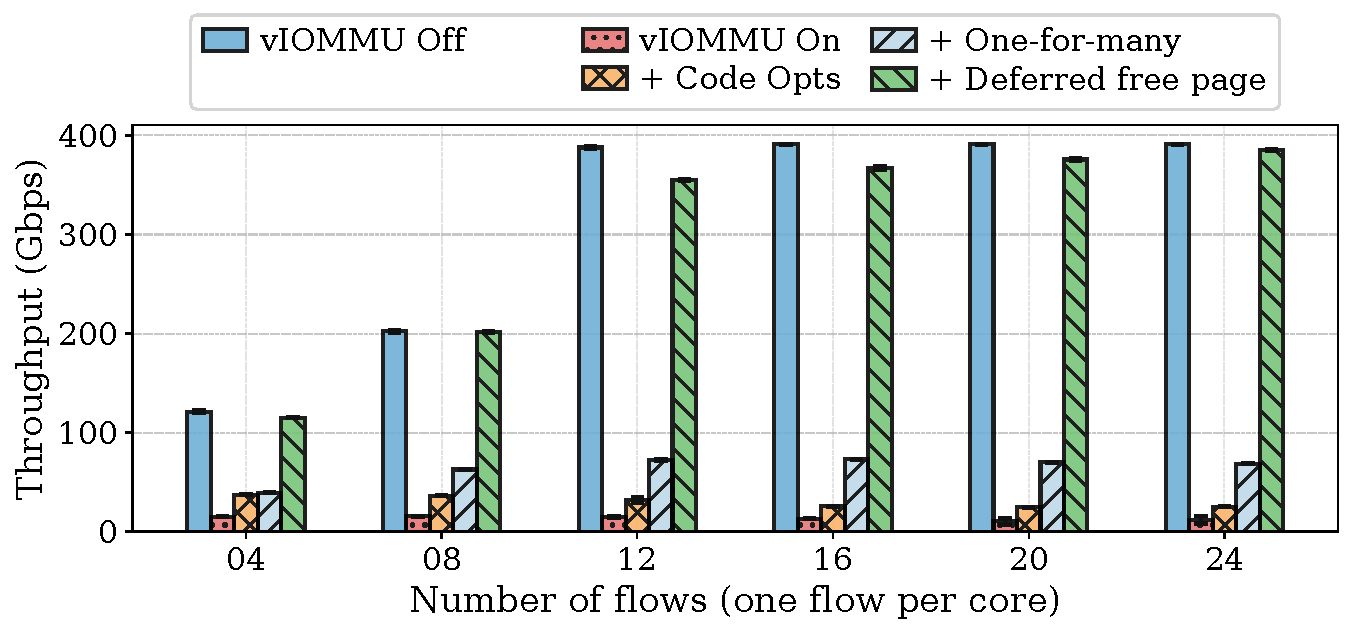
\includegraphics[width=0.95\textwidth]{figures/eval_ablation_tx-tput.pdf}
        \caption{Tx-server}
        \label{vfree:fig:ablation-tx}
    \end{subfigure}
    \begin{subfigure}[b]{\columnwidth}
        \centering
        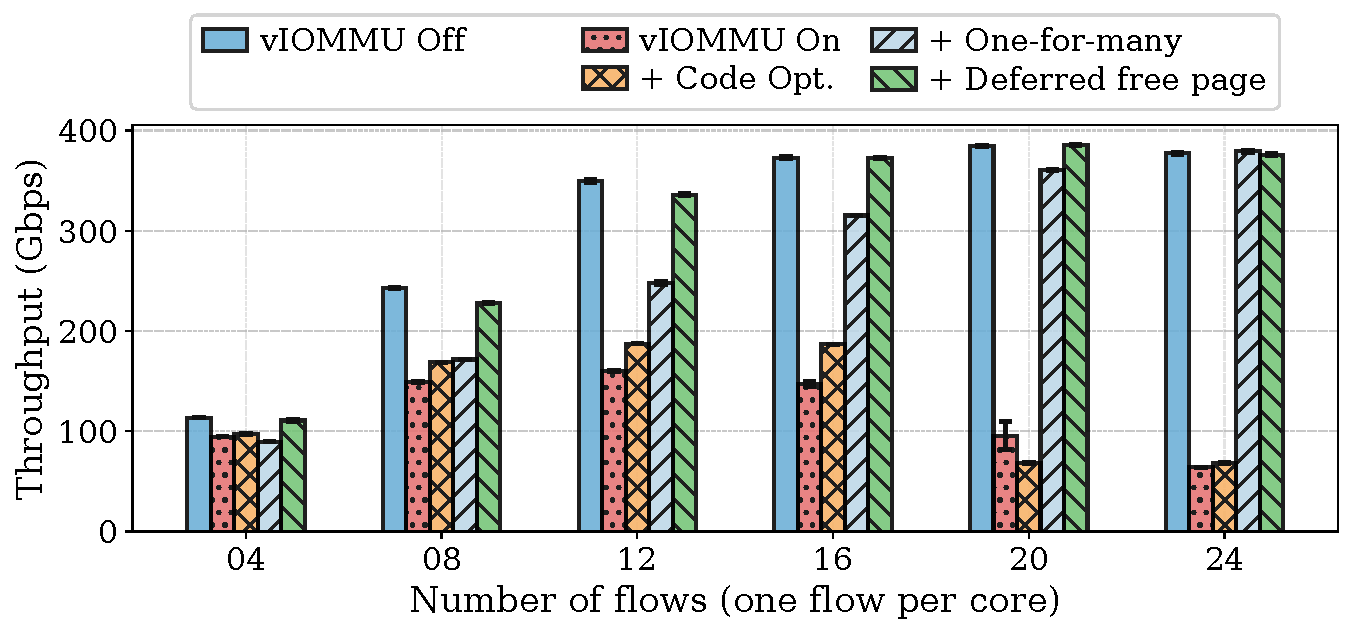
\includegraphics[width=0.95\textwidth]{figures/eval_ablation_rx-tput.pdf}
        \caption{Rx-server}
        \label{vfree:fig:ablation-rx}
    \end{subfigure}
    \caption{\small {\bf Necessity of both design ideas---one-for-many invalidations and deferred free page---to achieve {\vfreename} benefits.}}
    \label{vfree:fig:ablation}
\end{figure}

% \para{Difference between Rx and Tx behavior.} 
% The behavior of Tx contrasts with Rx,
% where datapath optimizations (\S\ref{vfree:sec:inefficiencies})\tianyin{???} reduce the number of invalidation requests,
%     resulting in smaller number of requests per batch (at most three).
% Hence, only a few cores are blocked at a time,
% and small batches are sufficient to amortize VM exit overhead.
% % and recover most of the lost performance.
% % \leshna{looking at both of them why do we not put tx first in both result and ablation study. It has better results and stronger argument of the need of both the design optimizations}

% With DFP, only the issuing core is blocked,
% while other cores can continue execution without stalling.
% Moreover, since unblocked cores can process more packets after enqueuing a request,
% \vfreebrand can batch more than one request per core and issue invalidation requests with larger batch sizes.
% Overall, \vfreebrand recovers the majority of the remaining throughput in the Tx case,
% improving performance by up to 5.6$\times$ over \optOne{}.

% \begin{figure}[!htbp]
%     \centering
%     \begin{subfigure}[b]{\columnwidth}
%         \centering
%         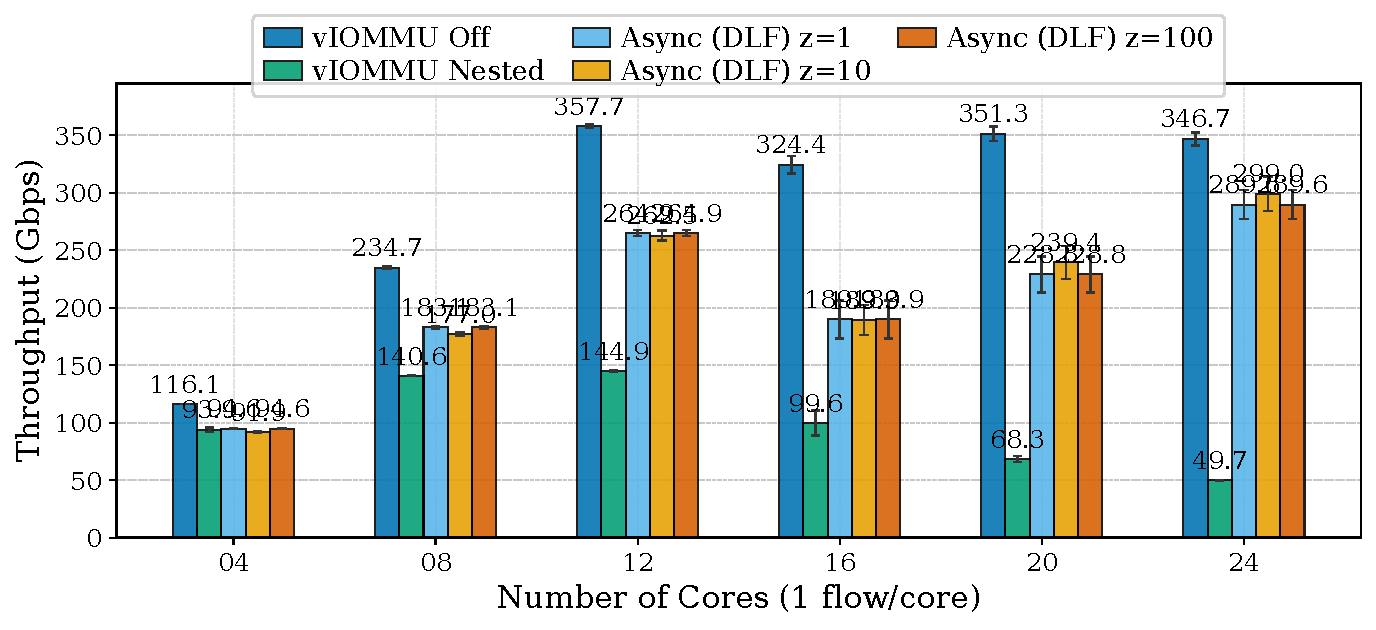
\includegraphics[width=\textwidth]{figures/eval_sensitivity_core_exp-tput.pdf}
%         \Description{Bar chart showing throughput sensitivity analysis when only Async Invalidation is enabled.}
%         \caption{Sensitivity Analysis when only Async Invalidation are enabled }
%         \label{vfree:fig:sensitivity-core}
%     \end{subfigure}
%     \vspace{1em}
%     \begin{subfigure}[b]{\columnwidth}
%         \centering
%         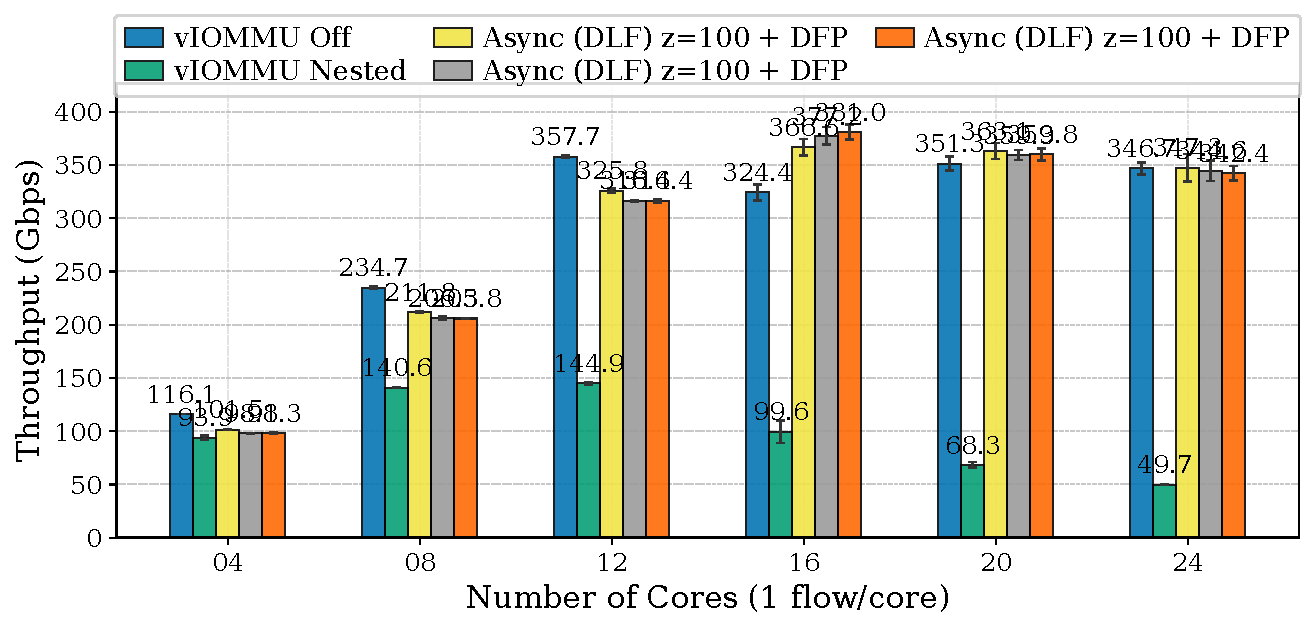
\includegraphics[width=\textwidth]{figures/eval_sensitivity_core_exp_dlf-tput.pdf}
%         \Description{Bar chart showing throughput sensitivity analysis when Async Invalidation is used with DFP.}
%         \caption{Sensitivity Analysis when only Async Invalidation is used in combination with DFP}
%         \label{vfree:fig:sensitivity-dlf}
%     \end{subfigure}
%     \caption{Parameter sensitivity of async invalidation implemented in distributed-leader-follower scheme.
%     Tested on with different maximum flushes per round (z=1, 10, 100)}
%     \label{vfree:fig:sensitivity}
% \end{figure}








\subsubsection{{\vfreename} Scalability with Increasing VM count}
\label{vfree:sec:eval-multi-vm}

Cloud deployments commonly deploy more than one VM per server.
We evaluate how {\vfreename} performance fares with an increasing number of VMs.
We fix the total core budget at 32 (the maximum per socket on our setup) and vary the number of VMs from 1 to 16, dividing the cores equally (\textit{e.g.}, assigning $32/N$ vCPUs) and using a dedicated SR-IOV Virtual Function~\cite{ms_sriov_overview} for each VM.
We report aggregate throughput across all VMs. {We focus on Tx-server setup since it shows the most severe degradation with vIOMMU-on.}


Figure~\ref{vfree:fig:multi-vm} shows that {\vfreename} maintains close-to-vIOMMU-off performance for each evaluated VM count,
while vIOMMU-on results in 80--96\% throughput degradation. As expected, with vIOMMU-on, aggregate throughput {increases} from 16.4\,Gbps with 1~VM to 75.8\,Gbps with 16~VMs.
{This is likely due to each VM independently being able to perform IR-SUB concurrently---increasing the arrival rate of IRs to the IOMMU invalidation queue.}

\begin{figure}[H]
    \centering
    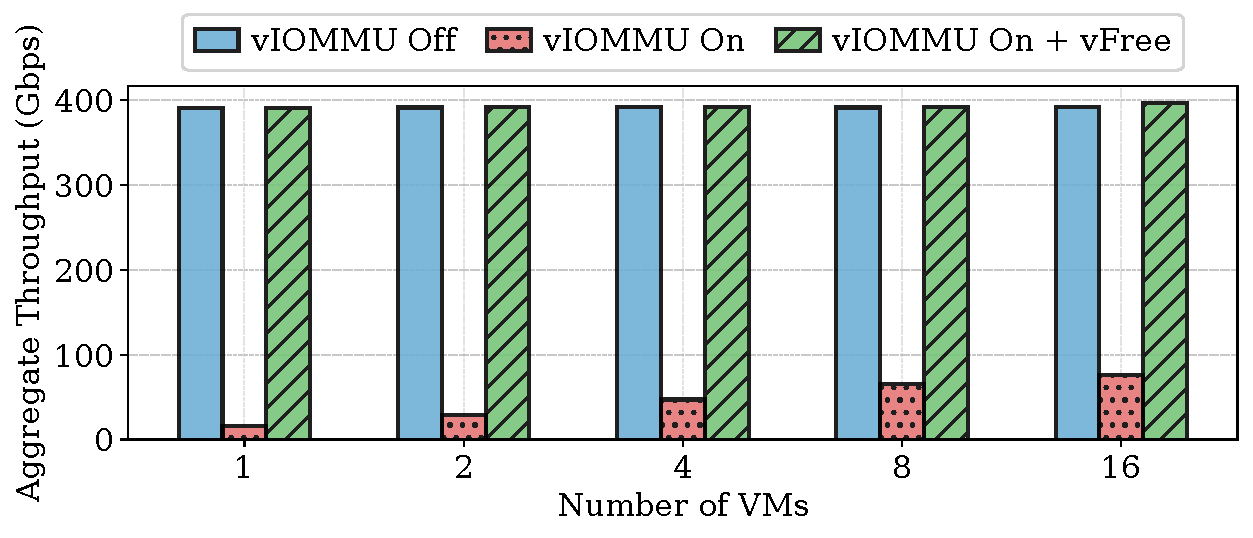
\includegraphics[width=0.75\columnwidth]{figures/many_vm_throughput.pdf}
    \caption{\small {\bf {\vfreename} maintains its benefits with increasing number of VMs per host. Discussion in \S\ref{vfree:sec:eval-multi-vm}}}
%    \vspace{-0.1in}
    \label{vfree:fig:multi-vm}
\end{figure}

% \saksham{Can we get rid of this-->}This is a direct consequence of the intra-VM contention structure identified in \S\ref{vfree:sec:inefficiencies}:
%     each VM has its own emulated invalidation queue,
%     so fewer cores per VM means less intra-VM serialization on the invalidation path.
% However, even in the best case (16~VMs), vIOMMU-on achieves only 19\% of vIOMMU-off throughput.
% {\vfreename} completely eliminates IOMMU overhead and scales well across multi-VM configurations, delivering $5.2$--$24\times$ improvement over vIOMMU-on.

\subsubsection{No Free Lunch: The Cost of {\vfreename} Benefits}
\label{vfree:ssec:cost}
{\vfreename} benefits come with two costs: it requires a dedicated core, and it requires extra memory due to deferred free page. We believe the former is not fundamental: it should be possible to opportunistically distribute the IR-SUB processing to producer threads (\textit{e.g.}, any lightly-loaded producer can become a consumer, and execute IR-SUB on its local core). Nevertheless, even with one dedicated core, {\vfreename} expands the choices of real-world systems: high performance but with weak (or no) IO memory protection, abysmal performance with \textit{significantly underutilized} cores with strict IO memory protection, or, high performance with one dedicated core with strict IO memory protection. For the extra memory, our evaluation results presented in the Appendix-B suggest that the extra memory requirements are less than $4\%$ across all our evaluated workloads.

% The cost of achieving {\vfreename} benefits is an additional core. 


% Cloud deployments commonly partition physical resources among multiple VMs. We evaluate how \vfreename{} performs as the same 32 cores are divided among an increasing number of VMs---from a single 32-vCPU VM to sixteen 2-vCPU VMs.

% We fix the total core budget at 32 and vary the number of VMs
% (1, 2, 4, 8, 16), assigning $32/N$ vCPUs to each of the $N$ VMs.
% Every VM has its own SR-IOV virtual function and runs under the
% same three configurations as in the single-VM experiments.
% We report the aggregate Tx throughput across all VMs.

% Figure~\ref{vfree:fig:multi-vm} shows that \vfreename{} matches vIOMMU-off
% performance at every VM count.
% In contrast, enabling vIOMMU without \vfreename{} causes
% 80--96\% throughput degradation depending on the VM count.

% With vIOMMU-on, aggregate throughput \emph{increases} from 16.4\,Gbps with 1~VM to 75.8\,Gbps with 16~VMs.
% This is a direct consequence of the per-VM contention structure identified in \S\ref{vfree:sec:inefficiencies}:
% each VM has its own emulated invalidation queue,
% so fewer cores per VM means less intra-VM serialization
% on the invalidation path.
% However, even in the best case (16 VMs),
% vIOMMU-on achieves only 19\% of vIOMMU-off throughput.
% \vfreename{} eliminates this bottleneck entirely,
% delivering up to 24$\times$ throughput improvement over vIOMMU-on (1~VM) and 5.2$\times$ at 16~VMs, where the baseline is least degraded.



% \subsubsection{Impact of Consumer Placement.}
% \todo{@Siyuan Add text}

%

